\documentclass{Article}
\usepackage[utf8]{inputenc}
\usepackage [danish]{babel}
\usepackage[a4paper, hmargin={2.8cm, 2.8cm}, vmargin={2.5cm, 2.5cm}]{geometry}
\usepackage{eso-pic} % \AddToShipoutPicture
\usepackage{graphicx} % \includegraphics
\linespread{1.2}
\usepackage{amsthm}
\usepackage{amsmath}
\usepackage{url}
\usepackage{tikz}
\usepackage{amsfonts}


\usepackage{listings}


\author{
\Large{dpj482}\\
    \\ \texttt{}
}

\title{
  \vspace{3cm}
  \Huge{CAC assignment 1} \\
  \Large{Christian Møllgaard}\\
}
\usepackage{natbib}
\usepackage{graphicx}

\begin{document}

%% Change `ku-farve` to `nat-farve` to use SCIENCE's old colors or
%% `natbio-farve` to use SCIENCE's new colors and logo.
%\AddToShipoutPicture*{\put(0,0){\includegraphics*[viewport=0 0 700 600]{natbio-farve}}}
\AddToShipoutPicture*{\put(0,602){\includegraphics*[viewport=0 600 700 1600]{natbio-farve}}}

%% Change `ku-en` to `nat-en` to use the `Faculty of Science` header
\AddToShipoutPicture*{\put(0,0){\includegraphics*{nat-en}}}

\clearpage\maketitle
\thispagestyle{empty}

%\newpage

%% Write your dissertation here.
\section{Changing the data structur}
Before the problem can be vectorised, the data structure containing the data needs to be vectorised. 
To make the best use of memory cahing i create my solar system and asteroids as two dimensional vectors, (7,n).
They have the dimension 7 first, so the values used at the same time, gets cached together.

As an example i show the new definition of the solar system array.
\lstinputlisting[language=Python, firstline=125, lastline=139]{nbodyphysics.py}

\section{What to vectorize}
The costly action in this script is the calc force function. This function is called on every object once for every planet there is using for loops. 

The main vetorizition goal is to remove these for loops. First challenge is to calculate the distance from every object to every other objet. This is done using ``newaxis''.
Then i need to fill the diagonal when comparing distance of planets to all planets, to make sure, there is no zero distance from planets to it self. I fill with the value 1, which is fine bacause the equation will be zero at the second half.
Then i calculate the mass difference like for every planet using newaxis.
Then i update the force of each planet for each dimension once at a time. This could be done using a one liner, but i found no gain from doin so, and this is easier to understand.

My calc force and move function ended up looking like this:
\lstinputlisting[language=Python, firstline=56, lastline=82]{nbodyphysics.py}


\section{Result}
Running the script on marge using the config file provided, i got these results:

\begin{table}[h!]
\centering
\caption{My caption}
\label{my-label}
\begin{tabular}{|l|l|l|l|l|}
\hline
bodies   & run 1         & run 2         & run 3         & avg           \\ \hline
1.00E+04 & 0.0949919224  & 0.0790441036  & 0.0791590214  & 0.0843983491  \\ \hline
1.00E+05 & 1.1335251331  & 1.0382509232  & 1.0500969887  & 1.0739576817  \\ \hline
1.00E+06 & 13.1345989704 & 12.4405839443 & 12.4634170532 & 12.6795333226 \\ \hline
\end{tabular}
\end{table}
The results provided for the sequential version:
\begin{table}[h!]
\centering
\caption{My results}
\label{my-label}
\begin{tabular}{|l|l|l|l|l|}
\hline
bodies   & run 1        & run 2        & run 3        & avg         \\ \hline
1E4 & 16,21 & 16,49 & 16,25 & 16,32 \\ \hline
1E5 & 161,89  & 165,88  & 163,16  & 163,65 \\ \hline
1E6 & 1616,78  & 1658,22  & 1627,89   & 1634,30 \\ \hline
\end{tabular}
\end{table}

Comparing the results of these two functions it's easy to see that there is a significant speed up using vectors. 
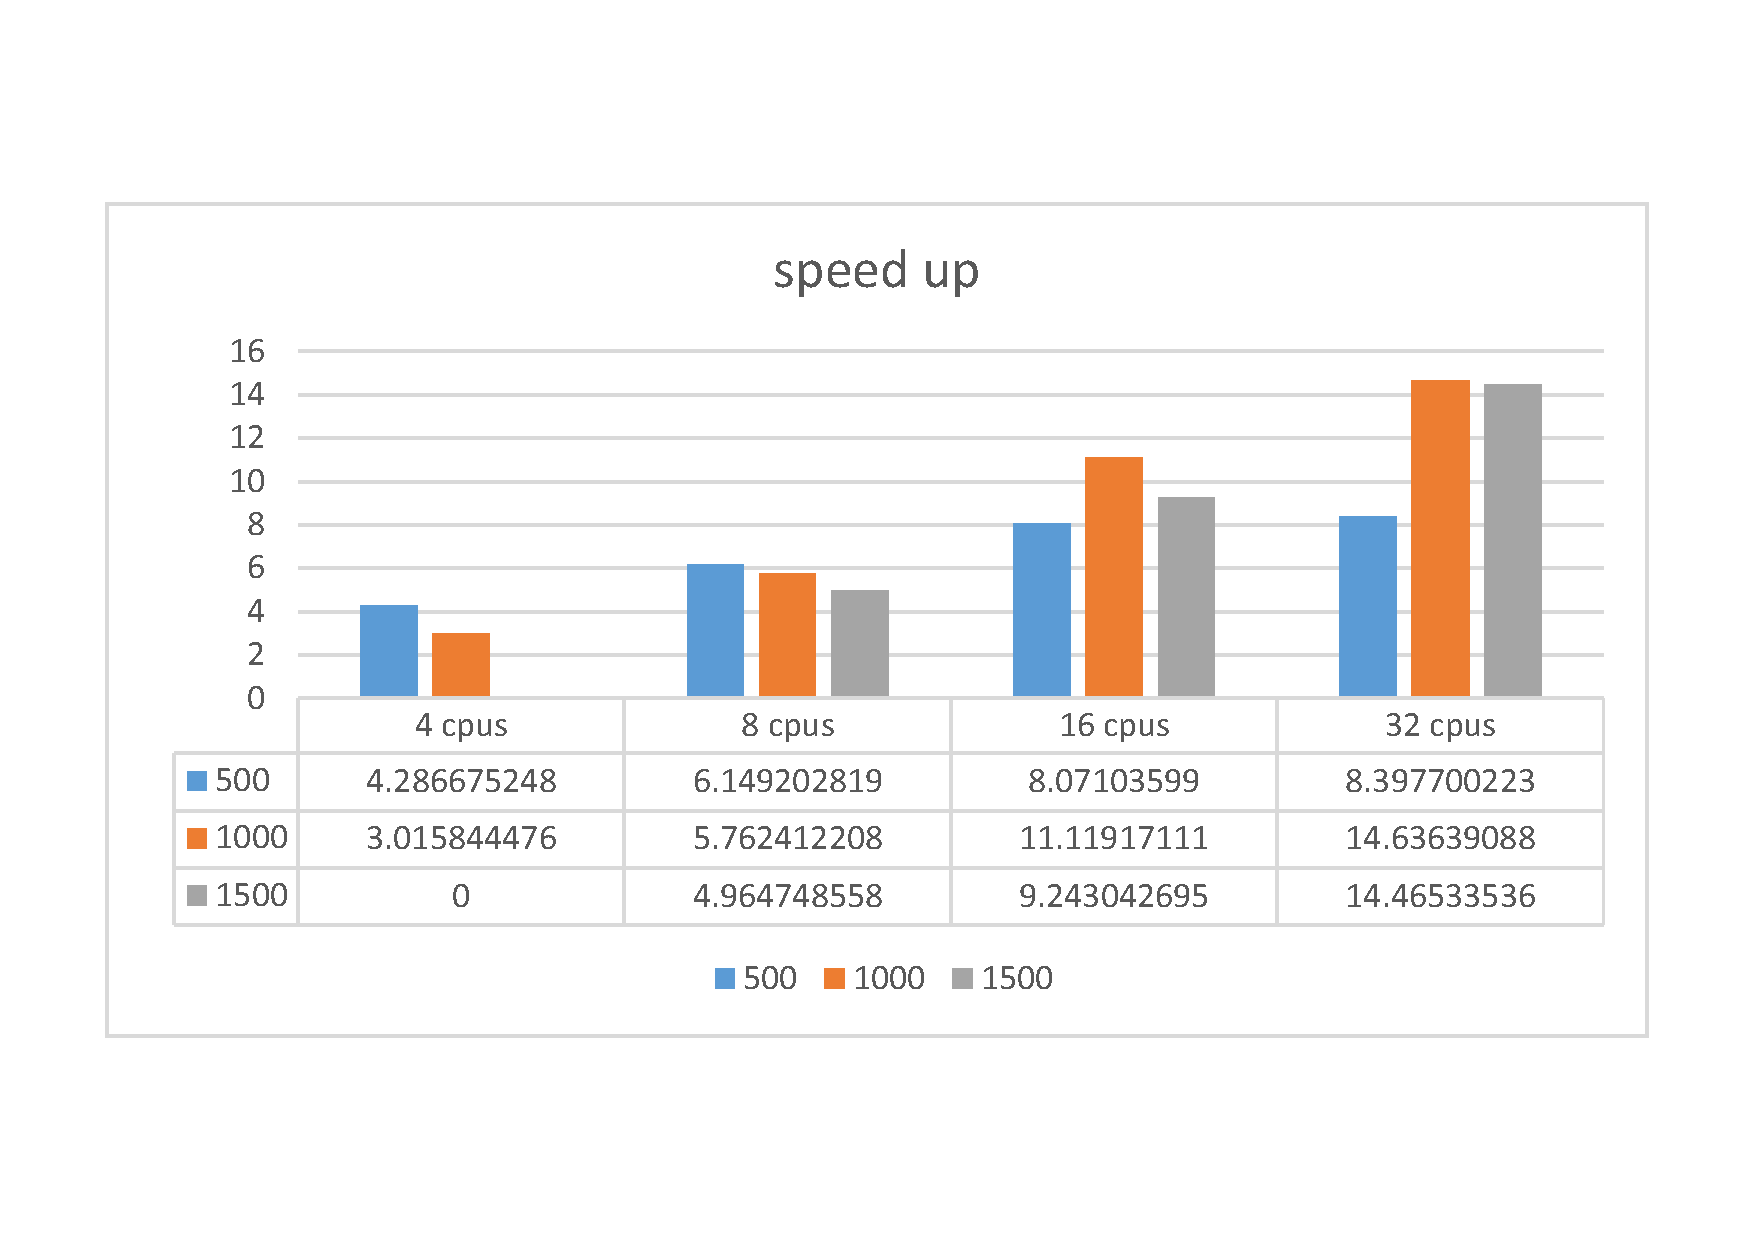
\includegraphics[scale=0.5]{speedup}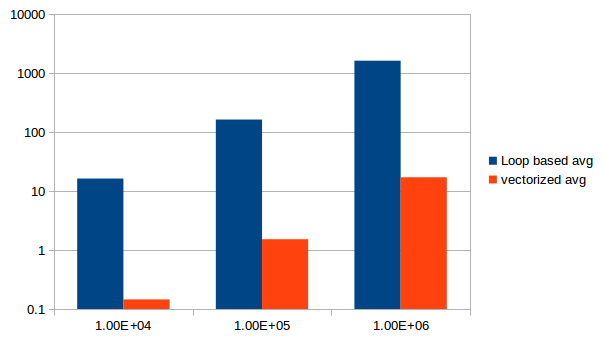
\includegraphics[scale=0.5]{runtime}

\end{document}
